%%%%%%%%%%%%%%%%%%%%%%%%%%%%%%%%%%%%%%%%%%%%%%%%%%%%%%%%%%%%%%%%%%%%%%%%%%%%%
%%%
%%% File: thesis.tex, version 1.9, May 2016
%%%
%%% =============================================
%%% This file contains a template that can be used with the package
%%% cs.sty and LaTeX2e to produce a thesis that meets the requirements
%%% of the Computer Science Department from the Technical University of Cluj-Napoca
%%%%%%%%%%%%%%%%%%%%%%%%%%%%%%%%%%%%%%%%%%%%%%%%%%%%%%%%%%%%%%%%%%%%%%%%%%%%%

\documentclass[12pt,a4paper,twoside]{report}         
\usepackage{cs}              
\usepackage{times}
\usepackage{graphicx}
\usepackage{latexsym}
\usepackage{amsmath,amsbsy}
\usepackage{amssymb}
\usepackage[matrix,arrow]{xy}
\usepackage[T1]{fontenc}
\usepackage{ae,aecompl}
\usepackage{romanian} %definitii pentru diacritice; 
\usepackage{amstext}
\usepackage{graphics}
\usepackage[T1]{fontenc}
\usepackage{ae,aecompl}
\usepackage{algorithm}
%\usepackage{algorithmic}
\usepackage{color}
\usepackage{color}

% \mastersthesis
\diplomathesis
% \leftchapter
\centerchapter
% \rightchapter
\singlespace
% \oneandhalfspace
% \doublespace

\renewcommand{\thesisauthor}{Alin Dan 'TANDEA}    %% Your name.
\renewcommand{\thesismonth}{Iunie}     %% Your month of graduation.
\renewcommand{\thesisyear}{2018}      %% Your year of graduation.
\renewcommand{\thesistitle}{Managementul studiilor clinice bazat pe
tehnologia blockchain} % Title
\renewcommand{\thesissupervisor}{asis. Ing. Cosmina Ivan}
\newcommand{\department}{FACULTATEA DE AUTOMATIC'A 'SI CALCULATOARE\\
DEPARTAMENTUL CALCULATOARE}
\newcommand{\thesis}{LUCRARE DE LICEN'T'A}
\newcommand{\uline}[1]{\rule[0pt]{#1}{0.4pt}}
%\renewcommand{\thesisdedication}{P'arin'tilor mei}
\newcommand{\utcnlogo}{
\includegraphics[width=15cm]{img/utcn.jpg}}

\begin{document}
%\frontmatter
%\pagestyle{headings}

\newenvironment{definition}[1][Defini'tie.]{\begin{trivlist}
\item[\hskip \labelsep {\bfseries #1}]}{\end{trivlist}}



%\thesistitle                    %% Generate the title page.
%\authordeclarationpage                %% Generate the declaration page.

\pagenumbering{arabic}
\setcounter{page}{4}



\begin{center}
%\includegraphics[width=15cm]{img/tucn.jpg}  
\utcnlogo

{\bf \department}

\vspace{4cm}

{\bf \thesistitle} %LICENSE THESIS TITLE}

\vspace{1.5cm}

\thesis

\vspace{6cm}

Absolvent: {\bf \thesisauthor} 

Conduc'ator 'stiin'tific: {\bf \thesissupervisor}

\vspace{3cm}
{\bf \thesisyear}
\end{center}

\thispagestyle{empty}
\newpage

\begin{center}
\utcnlogo

{\bf \department}
\end{center}
\vspace{0.5cm}

%\begin{small}
\begin{tabular}{p{7cm}p{8cm}}
 %\hspace{-1cm}& VIZAT,\\
 \hspace{-1cm}DECAN, & DIRECTOR DEPARTAMENT,\\
\hspace{-1cm}{\bf Prof. dr. ing. Liviu MICLEA} & {\bf Prof. dr. ing. Rodica POTOLEA}\\  
\end{tabular}
 
\vspace{2cm}

\begin{center}
Absolvent: {\bf \thesisauthor}

\vspace{1cm}

{\bf \thesistitle}
\end{center}

\vspace{1cm}

\begin{enumerate}
 \item {\bf Enun'tul temei:} {\it Scurt'a descriere a temei lucr'arii de licen't'a 'si datele ini'tiale}
\item {\bf Con'tinutul lucr'arii:} {\it (enumerarea p'ar'tilor componente) Exemplu: Pagina de prezentare, aprecierile coordonatorului de lucrare, titlul capitolului 1, titlul capitolului 2, titlul capitolului n, bibliografie, anexe.}
\item {\bf Locul document'arii:} {\it Exemplu}: Universitatea Tehnic'a din Cluj-Napoca, Departamentul Calculatoare
\item {\bf Consultan'ti:}
\item {\bf Data emiterii temei:} 1 Noiembrie 2016
\item {\bf Data pred'arii:} 21 Februarie 2018 {\it (se va completa data pred'arii)}
  \end{enumerate}
\vspace{1.2cm}

\hspace{6cm} Absolvent: \uline{6cm} 

\vspace{0.5cm}
\hspace{6cm} Coordonator 'stiin'tific: \uline{5cm} 
%\end{small}

\thispagestyle{empty}


\newpage
$ $
%\begin{center}
%\utcnlogo

%{\bf \department}
%\end{center}

\thispagestyle{empty}
\newpage

\begin{center}
\utcnlogo

{\bf \department}
\end{center}

\vspace{0.5cm}

\begin{center}
{\bf
Declara'tie pe proprie r'aspundere privind\\ 
autenticitatea lucr'arii de licen't'a}
\end{center}
\vspace{1cm}



Subsemnatul(a) \\
\uline{14.8cm}, 
legitimat('a) cu \uline{4cm} seria \uline{3cm} nr. \uline{4cm}\\
CNP \uline{9cm}, autorul lucr'arii \uline{2.8cm}\\
\uline{16cm}\\
\uline{16cm}\\
elaborat'a 'in vederea sus'tinerii examenului de finalizare a studiilor de licen't'a la Facultatea de Automatic'a 'si Calculatoare, Specializarea \uline{7cm} din cadrul Universit'a'tii Tehnice din Cluj-Napoca, sesiunea \uline{4cm} a anului universitar \uline{3cm}, declar pe proprie r'aspundere, c'a aceast'a lucrare este rezultatul propriei activit'a'ti intelectuale, pe baza cercet'arilor mele 'si pe baza informa'tiilor ob'tinute din surse care au fost citate, 'in textul lucr'arii 'si 'in bibliografie.

Declar, c'a aceast'a lucrare nu con'tine por'tiuni plagiate, iar sursele bibliografice au fost folosite cu respectarea legisla'tiei rom\ia ne 'si a conven'tiilor interna'tionale privind drepturile de autor.

Declar, de asemenea, c'a aceast'a lucrare nu a mai fost prezentat'a 'in fa'ta unei alte comisii de examen de licen't'a.

'In cazul constat'arii ulterioare a unor declara'tii false, voi suporta sanc'tiunile administrative, respectiv, \emph{anularea examenului de licen't'a}.

\vspace{1.5cm}

Data \hspace{8cm} Nume, Prenume

\vspace{0.5cm}

\uline{3cm} \hspace{5cm} \uline{5cm}

\vspace{1cm}
\hspace{9.4cm}Semn'atura

\thispagestyle{empty}

\newpage


%\listoftables
%\listoffigures

%\clearpage 
%\newpage

%\begin{comment}
{\color{red}{\bf De citit 'inainte} (aceast'a pagin'a se va elimina din versiunea final'a)}:
\begin{enumerate}
 \item Cele trei pagini anterioare (foaie de cap'at, foaie sumar, declara'tie) se vor lista pe foi separate (nu fa't'a-verso), fiind incluse 'in lucrarea listat'a. 
 Foaia de sumar (a doua) necesit'a semn'atura absolventului, respectiv a coordonatorului.
 Pe declara'tie se trece data c\ia nd se pred'a lucrarea la secretarii de comisie.
 \item Pe foaia de cap'at, se va trece corect titulatura cadrului didactic 'indrum'ator, 'in englez'a (consulta'ti pagina de unde a'ti desc'arcat acest document pentru lista cadrelor didactice cu titulaturile lor).
 \item Documentul curent {\bf nu} a fost creat 'in MS Office. E posibil sa fie mici diferen'te de formatare. 
\item Cuprinsul 'incepe pe pagina nou'a, impar'a (dac'a se face listare fa't'a-verso), prima pagin'a din capitolul Introducere tot a'sa, fiind numerotat'a cu 1. % Pentru actualizarea cuprinsului, click dreapta pe cuprins (zona cuprinsului va apare cu gri), Update field-$>$Update entire table.
\item Vizualiza'ti (recomandabil 'si 'in timpul edit'arii) acest document % după ce activaţi vizualizarea simbolurilor ascunse de formatare (apăsaţi simbolul  din Home/Paragraph).
\item Fiecare capitol 'incepe pe pagin'a nou'a. % datorită simbolului ascuns Section Break (Next Page) care este deja introdus la capitolul precedent. Dacă ştergeţi din greşeală simbolul, se reintroduce (Page Layout -> Breaks).
\item Folosi'ti stilurile predefinite (Headings, Figure, Table, Normal, etc.)
\item Marginile la pagini nu se modific'a.
\item Respecta'ti restul instruc'tiunilor din fiecare capitol.
\end{enumerate}
 
%\end{comment}

\newpage

\tableofcontents
\newpage



\chapter{Introducere - Contextul proiectului}
\pagestyle{headings}

Titlul capitolului se bazeaz'a pe Heading 1 style, numerotat cu o cifra (x. Nume capitol), font Times New Roman de 14, Bold.

Ce se scrie aici:

\begin{itemize}
 \item Contextul
\item Conturarea domeniului exact al temei
\item Reprezint'a cca. 5\% din lucrare
\end{itemize}


\section{Contextul proiectului}

Fontul folosit implicit 'in acest document este Times New Roman, dimensiune de 12, conform Normal style, cu spa'tiere la 1 r\ia nd (Paragraph, Line spacing de 1.0) 'si Justify. 
Pentru prima linie din fiecare paragraf se folose'ste indentare (implicit 'in Normal Style), iar 'intre paragrafe succesive nu se las'a distan't'a suplimentar'a\footnote{Sunt rezolvate automat de Latex}.

\subsection{Subsection}
Fiecare tabel introdus 'in lucrare este numerotat astfel: Tabel x.y, unde x reprezint'a num'arul capitolului iar y num'arul tabelului din capitol. 
Se las'a un r\ia nd liber 'intre tabel 'si paragraful anterior, respectiv posterior (table~\ref{table:nonlin}).

\begin{table}[ht]
\caption{Rezultate}
\centering                          % tabel centrat 
\begin{tabular}{|c|c|c|c|}          % 4 coloane centrate 
\hline\hline                        % linie orizontala dubla
Case & Method\#1 & Method\#2 & Method\#3 \\ [0.5ex]   % inserare tabel
%heading
\hline                              % linie orizontal simpla
1 & 50 & 837 & 970 \\               % corpul tabelului 
2 & 47 & 877 & 230 \\
3 & 31 & 25 & 415 \\[1ex]           % [1ex] adds vertical space
\hline                              
\end{tabular}
  % titlul tabelului
\label{table:nonlin}                % \label{table:nonlin} introduce eticheta folosita pentru referirea tabelului in text; referirea in text se va face cu \ref{table:nonlin}
\end{table}

Fiecare figur'a introdus'a 'in text este citat'a (de ex: 'in figura x.y este prezentat'a ...) 'si numerotat'a. 
Numerotarea se face astfel Figura x.y unde x reprezint'a num'arul capitolului iar y num'arul figurii 'in acel capitol. 
E.g.: figure~\ref{fig:imag}.

\begin{figure}[ht]
    \centering
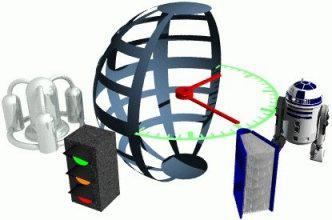
\includegraphics[]{img/test.jpg}
    \caption{Numele figurii}
    \label{fig:imag}
\end{figure}

Fiecare capitol 'incepe pe pagin'a nou'a.

\chapter{Obiectivele Proiectului}

'In acest capitol se prezint'a tema propriu-zis'a (sub forma unei teme de proiectare sau cercetare, formulat'a exact, cu obiective clare - 2-3 pagini 'si eventuale figuri explicative).

Reprezint'a cca. 10\% din lucrare.
\section{Titlu}
\section{Alt titlu}

\chapter{Studiu Bibliografic}
	In acest capitol sunt prezentate o serie de concepte si tehnologii necesare pentru o mai buna intelegere a temei alese si a modului in care au fost utilizate pentru implementarea acesteia. Capitolul continua prin descrierea aplicarii acestor concepte in anumite domenii precum si in domeniul studiilor clinice. Sunt prezentate unele beneficii aduse de aceste tehnologii, alaturi de o comparatie a implementarilor existente ale acesteia.
	\section{Blockchain}	
	Termenul de blockchain a devenit cunoscut odata cu cresterea in popularitate a monedelor virtuale, in special a monedei virtuale Bitcoin. O retea blockchain poate fi definita ca fiind o baza de date distribuita, intretinuta de o serie de participanti care valideaza inregistrarile din cadrul retelei folosind o comunicare de tip peer-to-peer. Inregistrarile din cadrul retelei sunt securizate prin metode criptografice care asigura imutabilitatea datelor. Rezolvarea conflictelor care pot aparea intre inregistrarile din retea are loc prin utilizarea unor algoritmi de consens. Aceasta sectiune analizeaza urmatoarele aspecte ale tehnologiei: structura de date, aspecte legate de criptografie, topologia retelei, algoritmi de consens, smart contracts, permisiuni si implementari ale tehnologiei.

	\subsection{Structura de date}
	Structura de date folosita reprezinta unul dintre mijloacele care asigura integritatea datelor din reteaua blockchain. Documentatia monedei virtuale Bitcoin descrie structura de date folosita ca fiind o lista invers inlantuita in care fiecare element, numit bloc, contine contine hash-ul blocului anterior, un timestamp si radacina Merkle a tranzactiilor, folosita pentru a verifica integritatea acestora. Figura \ref{fig:btc} prezinta structura de date folosita de Bitcoin\cite{bitcoin}. \\
	
		\begin{figure}[H]
		\begin{center}
			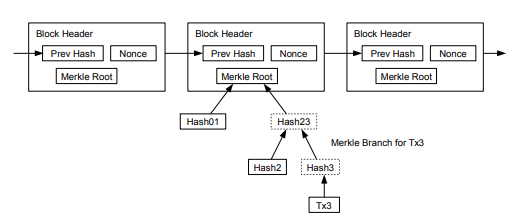
\includegraphics[scale=2.5]{img/btc.png}
			\caption{Cel mai lung lan't proof-of-work folosit de Bitcoin\cite{bitcoin}}
  			\label{fig:btc}
  		\end{center}
  		\end{figure} 
	
	Fiecare bloc din structura de date este identificat prin functia hash a header-ului blocului curent si a blocului anterior. Conceptul implementat de moneda virtuala Bitcoin este urmat de alte implementari care au adus unele modificari acestei structuri, dar pastreaza unele concepte de baza introduse de Bitcoin. 
	\subsection{Topologia re'telei}
	O caracteristica importanta a unei retele blockchain este lipsa unei autoritati centrale care sa intermedieze tranzactiile din cadrul retelei. Pentru validarea si propagarea tranzactiilor este folosita o retea peer-to-peer de participanti\cite{p2p}. In cadrul unei astfel de retele fiecare participant are aceleasi responsabilitati si privilegii, spre deosebire de o topologie client-server unde reteaua are un nod central cu capabilitati si responsabilitati diferite fata de clientii din retea. Figura \ref{fig:p2p} ilustreaza diferenta dintre cele doua toplogii.
			\begin{figure}[H]
		\begin{center}
			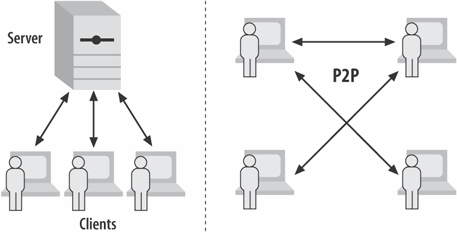
\includegraphics[scale=2]{img/p2p.png}
			\caption{Retea client-server vs peer-to-peer\cite{fabricdoc}}
  			\label{fig:p2p}
  		\end{center}
  		\end{figure}
Fiecare peer detine o copie a informatiilor din retea. Acest lucru face dificila modificarea abuziva a datelor, orice modificare fiind vizibila pentru ceilalti participanti.   
\subsection{Func'tii de hash si criptografie}
	O functie de hash reprezinta o metoda unidirectionala de mapare a unui sir de caractere de lungime arbitrara la un sir de caractere cu lungime fixa. Proprietatile necesare pentru o functie de hash sunt:
	\begin{itemize}
		\item Calcul rapid: efortul computational pentru calcularea rezultatului trebuie sa fie mic indiferent de sirul de intrare.
		\item Unidirectionala: obtinerea sirului original din hash nefezabila
		\item Determinista: rezultatul pentru un anumit sir de intrare este acelasi indiferent de cate ori este calculat. 
		\item Rezistent la coliziuni: oricare ar fi sirurile de intrare a,b functia de hash h(a) = h(b) doar daca a = b. Cu alte cuvinte un sir de intrare produce intotdeauna un rezultat unic.
		\item Schimbarile mici din sirul de intrare produc schimbari majore in rezultatul functiei de hash
\end{itemize}		
	 Printre algoritmii de hash folositi de diferitele implementari ale tehnologie blockchain se numara SHA256(Bitcoin) sau Keccak-256(Ethereum). Aceste functii sunt folosite si de catre algoritmii pentru stabilirea consensului.\\
		Pentru controlarea accesului in reteaua blockchain este folosita metoda de criptografie cu cheie publica. Aceasta presupune folosirea unei perechi de chei formata dintr-o cheie privata si o cheie publica, derivata din cheia privata. Pentru autorizarea tranzactiilor este folosita partea privata a cheii. Identitatea unui utilizator este data de partea publica a cheii. 
		\subsection{Mecanism de consens}
		O proprietate importanta a unei retele blockchain este lipsa unei autoritati centrale care sa valideze tranzactiile efectuate de participanti. Din aceasta cauza apare nevoia existentei unor mecanisme responsabile de rezolvarea conflictelor care apar in cadrul retelei intre inregistrarile detinute de participantii din retea. Algorimii de consens cei mai folositi sunt: Proof of Work(PoW) si Bizantine Fault Tolerance(BFT).
	
		PoW este algoritmul aflat in spatele unor monede virtuale precum Bitcoin si Ethereum. Algoritmul este conceput sub forma unei competitii in care participantii din retea isi folosesc puterea de calcul pentru rezolvarea unei probleme. Primul participant care rezolva problema primeste dreptul de a crea urmatorul bloc din structura de date alaturi de o anumita recompensa. Rezolvarea problemei presupune efort masiv de calcul si din acest motiv este folosita drept masura de siguranta. Pentru a modifica intrarile deja salvate in blockchain un atacator are nevoie de mai mult de 50\% din puterea de calcul a intregii retele, un astfel de atac fiind nefezabil. In acest mod este asigurata corectitudinea informatiilor insa metoda folosita este ineficienta.
		
		BFT asigura ajungerea la consens in cazul in care o parte din patricipanti sunt atacatori. Un algorimt pentru problema  cunoscuta sub numele de "Problema generalilor bizantini" a fost implementat in anul 1999 Miguel Castro and Barbara Liskov sub numele de Practical Bizantine Fault Tolerance(PBFT). Algoritmul incearca ajungerea la un consens in cadrul sistemului, pastrand in acelasi timp o laten'ta scazuta si eficienta ridicata. Pasii algoritmului sunt urmatorii:
		\begin{itemize}
			\item Un client trimite o cerere 
			\item Cererea este transmisa celorlalti clienti
			\item Ceilalti clienti executa cererea si transmit raspunsul clientului care a initiat cererea
			\item Clientul asteapta pana cand primeste F + 1 raspunsuri identice, unde F este numarul maxim de noduri malitioase tolerate
			
		\end{itemize}
		Conditia pentru functionarea corecta a sistemului este ca numarul de noduri malitioase din sistem sa fie mai mic decat 1/3 din numarul total de noduri din sistem.
		
		O comparatie la nivel inalt a celor doua mecanisme de stabilire a consensului este prezentata in tabelul \ref{table1}. Tabelul prezinta o comparatie a celor doi algoritmi luand in considerare unele proprietati importante ale unei retele blockchain: identitatea nodurilor, performanta, scalabilitatea, rezistenta la atacuri sau puterea consmata.
	 
	% Please add the following required packages to your document preamble:
% \usepackage[normalem]{ulem}
% \useunder{\uline}{\ul}{}
\begin{table}[H]
\centering
\caption{Comparatie la nivel inalt: PoW vs BFT}
\label{table1}
\begin{tabular}{|l|l|l|llll}
\cline{1-3}
                                                                                 & Proof of Work                                                                                  & Bizantine Fault Tolerance                                                                                        &  &  &  &  \\ \cline{1-3}
\begin{tabular}[c]{@{}l@{}}Managementul \\ identitatii \\ nodurilor\end{tabular} & deschis, decentralizat                                                                         & \begin{tabular}[c]{@{}l@{}}fiecare nod trebuie \\ sa cunoasca informatii \\ despre celelalte noduri\end{tabular} &  &  &  &  \\ \cline{1-3}
Scalabilitate                                                                    & excelenta                                                                                      & limitata                                                                                                        &  &  &  &  \\ \cline{1-3}
Performanta(throuput)                                                            & limitata                                                                                       & \begin{tabular}[c]{@{}l@{}}excelenta(mii de \\ tranzactii/sec)\end{tabular}                                      &  &  &  &  \\ \cline{1-3}
Performanta(laten'ta)                                                            & latenta crescuta                                                                               & \begin{tabular}[c]{@{}l@{}}excelenta(similara \\ cu cea indusa de retea)\end{tabular}                            &  &  &  &  \\ \cline{1-3}
Putere consumata                                                                 & \begin{tabular}[c]{@{}l@{}}Ridicata(PoW \\ necesita putere \\ de calcul ridicata)\end{tabular} & Scazuta                                                                                                          &  &  &  &  \\ \cline{1-3}
\begin{tabular}[c]{@{}l@{}}Numar total \\ de atacatori tolerati\end{tabular}     & \begin{tabular}[c]{@{}l@{}}\textless{}25\% din puterea \\ de calcul\end{tabular}               & \begin{tabular}[c]{@{}l@{}}\textless{}33\% din numarul\\  de noduri care voteaza\end{tabular}                    &  &  &  &  \\ \cline{1-3}
\end{tabular}
\end{table}		

Se poate observa faptul ca algoritmii reprezinta doua abordari diferite in cadrul unei retele blockchain. PoW pune accent pe scalabilitate dar prezinta o performanta scazuta in tim ce BFT asigura performanta ridicata dar cu o scalabilitate redusa. Decizia in ce priveste tipul de algoritm folosit depinde de nevoia sistemelor implementate.
	\subsection{Smart comtract}
	Un smart contract reprezinta "un set de promisiuni in format digital in care partile implicate actioneaza conform acestor promisiuni". Altfel spus aceste contracte sunt o reprezentare digitala a unor clauze contractuale, integrate in software pentru a media actiuni prin operatii bazate pe reguli. Odata ce preconditiile pentru un smart contract sunt indeplinite si acesta este initiat actiunile din cadrul lui sunt executate, ele fiind irevocabile.
	\subsection{Implementari ale tehnologiei blockchain}
	Prima implementare cu succes a tehnologiei blockchain a fost realizata de moneda virtuala bitcoin. Odata cu cresterea acesteia in popularitate au aparut diverse implementari ale acestei tehnologii, fiecare avand unele particularitati si scopuri de utilizare diferite.
	
	
	Tipuri de implementari. Exista 3 tipuri de implementari ale tehnologiei blockchain: public, privat si bazat pe permisiuni. Tabelul \ref{table2} prezinta o analiza la nivel inalt a celor 3 tipuri de implementari. Sunt luate in considerare aspecte precum drepturile de acces, performanta, costurile implicate, avantajele si dezavantajele fiecarei implementari precum si numarul de puncte de esec in cazul fiecareia.
	
	Blockchain public. In cadrul unu blockchain public nu exista nevoia definirii unor  drepturi de acces. Orice entitate are drepturi de acces egale in cadrul retelei si poate participa la procesul de validare a tranzactiilor. Din acest punct de vedere un blockchain public foloseste o topologie decentralizata nefiind prezenta o autoritate centrala care sa medieze tranzactiile din retea. O astfel de implementare este folosita de catre monedele virtuale Bitcoin sau Ethereum. In cadrul acestor retele participantii efectuaza tranzactii fara a fi implicata a treia entitate in acest proces. Pentru a se ajunge la un consens, un mecanism de tip PoW este folosit, acesta avand un impact asupra performantei retelei si a consumului de enegie.
	
	Blockchain privat. Spre deosebire de un blockchain public, cel privat foloseste o topologie centralizata. Accesul la retea este controlat de o autoritate centrala, aceasta avand dreptul de a lua decizii si de a implementa reguli in cadrul retelei. Un astfel de blockchain poate fi folosit in cazul in care este necesara restrictionarea accesului publicului larg la retea. O astfel de retea se bazaza pe stabilirea unui nivel ridicat de incredere in autoritatea centrala responsabila de administrarea retelei. Deoarece doar o singura entitate este responsabila de procesul de validare a tranzactiilor, apare avantajul performantei crescute in comparatie cu un blockchain public.
	
	Blockchain bazat pe permisiuni. Acesta abordare poate fi vazuta ca n hibrid intre un blockchai privat si unul public. Autoritatea in retea este detinuta de un set de entitati care pot face parte din organizatii diferite. Aceste entitati stabilesc dreptrile de acces la retea si rparticipa la validarea tranzactiilor. Drepturile de acces depind de identitatile participantilor, fiind nevoie de executarea unor smart contracts inainte de executarea unor tranzactii pentru validarea identitatii participantilor. Hyperledger Fabric si Corda sunt implementari ale unui astfel de blockchain. Ambele sunt solutii open-source care pot fi folosite pentru stocarea si partajarea datelor intre participantii retelei.
\begin{table}[]
\caption{Comparatie la nivel inalt a implementarilor tehnologiei blockchain}
\label{table2}
\resizebox{\textwidth}{!}{%
\begin{tabular}{|l|l|l|l|}
\hline
                                                          & Public                                                                                                                                                                                                             & Privat                                                                                                                                                                                    & Bazat pe permisiuni                                                                                                                                                                                                                                                   \\ \hline
Topologie retea                                           & decentralizata                                                                                                                                                                                                     & \begin{tabular}[c]{@{}l@{}}partial\\ decentralizata\end{tabular}                                                                                                                          & \begin{tabular}[c]{@{}l@{}}partial\\ decentralizata\end{tabular}                                                                                                                                                                                                      \\ \hline
Definire                                                  & \begin{tabular}[c]{@{}l@{}}Oricine are acces \\ la datele din retea. \\ Toate nodurile \\ participa la validare\end{tabular}                                                                                       & \begin{tabular}[c]{@{}l@{}}Permisiunile de acces \\ sunt controlate de o \\ singura entitate de \\ incredere din retea\end{tabular}                                                       & \begin{tabular}[c]{@{}l@{}}Permisiunile de acces\\ sunt controlate de un \\ numar prestabilit \\ de noduri cu autoritate\end{tabular}                                                                                                                                 \\ \hline
Beneficii                                                 & \begin{tabular}[c]{@{}l@{}}- Sigur, deoarece toti \\ participantii contribuie \\ la validarea tranzactiilor\\ - Transparent, toate \\ tranzactiile fiind publice\\ iar entitatile implicate\\ anonime\end{tabular} & \begin{tabular}[c]{@{}l@{}}- Verificare eficienta \\ a tranzactiilor de catre\\ autoritatea centrala\\ - Autoritatea centrala \\ decide entitatile care \\ au acces la retea\end{tabular} & \begin{tabular}[c]{@{}l@{}}- Eficient, deoarece un\\ numar relativ mic de\\ noduri verifica tranzactiile\\ - Drepturile de acces sunt \\ controlate de un set \\ predeterminat de noduri\\ - Controlul nu este detinut \\ de catre o autoritate centrala\end{tabular} \\ \hline
Provocari                                                 & Eficienta scazuta                                                                                                                                                                                                  & \begin{tabular}[c]{@{}l@{}}Controlul este detinut\\ de o singura entitate\end{tabular}                                                                                                    &                                                                                                                                                                                                                                                                       \\ \hline
Cost                                                      & scazut                                                                                                                                                                                                             & ridicat                                                                                                                                                                                   & mediu                                                                                                                                                                                                                                                                 \\ \hline
Performanta                                               & scazuta                                                                                                                                                                                                            & excelenta                                                                                                                                                                                 & ridicata                                                                                                                                                                                                                                                              \\ \hline
\begin{tabular}[c]{@{}l@{}}Puncte de \\ esec\end{tabular} & n                                                                                                                                                                                                                  & 1                                                                                                                                                                                         & * (nodurile cu autoritate)                                                                                                                                                                                                                                            \\ \hline
\end{tabular}%
}
\end{table}

\section{Scenarii de utilizare ale tehnologiei blockchain}
Sectiunea curenta descrie unele sisteme existente care au la baza implementarii lor tehnologia blockchain. Capitolul prezinta motivatia alegerii tehnologiei blockchain precum si avantajele aduse de aceasta in sistemele implementate

\subsection{Determinarea identitatii digitale}

In lucrarea [cite here] autorul incearca obtinerea un sistem pentru managementul identitatii digitale a utilizatorilor care sa aiba urmatoarele proprietati:
\begin{itemize}
	\item \textbf{Existenta} : entitatile trebuie sa existe independent, nu doar in mediul digital
	\item \textbf{Control}: o entitate are controlul absolut asupra identitatii proprii
	\item \textbf{Transparenta}: sistemele care mentin actualizata identitatea trebuie sa realizeze aceasta in mod transparent
	\item \textbf{Portabilitate} : identitatea trebuie sa fie transportabila
	\item \textbf{Consimtamant} : entitatile trebuie sa fie de acord cu partajarea informatiilor personale inainte de efectuarea acesteia.
\end{itemize}


Lucrarea propune un sistem decentralizat bazat pe tehnologia blockchain pentru managementul indetitatii consumatorilor, fiind implicate institutiile care emit identitatea si cele care se folosesc de aceasta. Beneficiile aduse de utilizarea tehnologiei blockchain in acest sistem sunt: schimbul decentralizat de informatii legate de identitatea unei persoane, partajarea informatiilor doar cu acordul clientului care detine identitatea, independenta fata de entitatea care a emis o anumita informatie legata de identitatea unui client.

\subsection{Trasarea provenientei produselor}

Lucrarea [cite here] prezinta un sistem care are ca scop urmarirea distributiei, originii si a starii curente a produselor intr-un mediu complex care implica un numar ridicat de participanti din diferite organizatii. Solutia propusa foloseste framework-ul Hyperledger Fabric pentru implementarea unei retele decentralizate care sa faciliteze si sa imbunatateasca transparenta si posibilitatea de urmarire a originii produselor.

\section{Tehnologia blockchain in studiile clinice}
Tehnologia blockchain poate avea un impact global asupra cercetarii clinice deoarece permite urmarirea, partajarea si protectia informatiilor. Prin utilizarea unui sistem decentralizat folosit pentru urmarirea activitatilor din cadrul unui studiu clinic si a unei retele peer-to-peer pentru partajarea informatiilor sunt asigurate transparenta si protectia datelor personale ale pacientilor. Un sistem bazat pe aceasta tehnologie poate imbunatati metodologiile din cercetarea clinica si protectia datelor cu caracter sensibil.

\subsection{Motivatie}


\subsection{Modelarea cercetarii clinice sub forma unei retele de afaceri}

	O \textbf{retea de afaceri} reprezint'a o re'tea complex'a de companii "unde scopul este de a sus'tine cerintele informationale 'si opera'tionale ale afacerii cum ar fi cele de marketing, contabilitate ..."\cite{bndef}. Un alt aspect important al unei retele de afaceri este ca aceasta nu inglobeaza doar afacerea in sine ci implic'a 'si unele entitati din exterior care sus'tin activitatea re'telei cum ar fi furnizorii sau distribuitorii. 
	
	In cazul studiilor clinice o retea de afaceri poate fi format'a din participan'tii direc'ti la activita'ti(ex. centrele medicale in care se desfasoar'a studiile clinice), precum si partile care sustin activitatea studiilor clinice(ex. furnizori, institutii de reglementare...)
	Re'telele existente de afaceri folosesc in prezent metode similare pentru stocarea informa'tiilor. Entit'atile implicate tranzactioneaza intre ele, 'ins'a men'tin inregistrari proprii referitoare la tranzactiile efectuate. In cele mai multe cazuri o autoritate central'a in care toate partile implicate au incredere intermediaz'a tranzactiile 'si schimbul de informa'tii din cadrul re'telei. Conceptul descris mai sus este ilustrat in figura \ref{fig:centralised}.\\	
		\begin{figure}[!ht]
		\begin{center}
			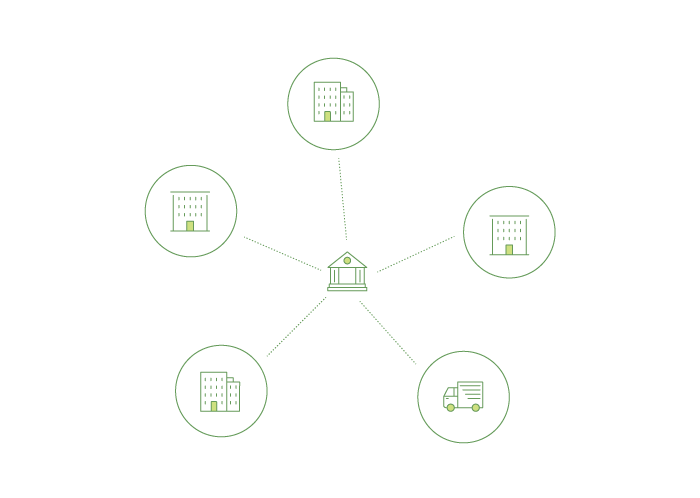
\includegraphics[scale=1.60]{img/current_network.png}
			\caption{Re'tele de afaceri centralizate\cite{fabricdoc}}
  			\label{fig:centralised}
  		\end{center}
  		\end{figure}
  		
	Aceasta metod'a prezint'a o complexitate redus'a dar produce in acelasi timp unele dezavantaje. Partajarea informatiilor este efectuata indirect, responsabila de acest lucru fiind autoritatea centrala. Din acest motiv procesul este incetinit, implicand costuri suplimentare. Stabilirea corectitudinii informatiilor devine dificila in momentul in care partile implicate detin inregistrari diferite referitoare la tranzactii.
		Printre sistemele care folosesc o astfel de abordare se numar'a Oracle Siebel Clinical Trial Management System\cite{ctms}. Sistemul ofer'a posibilitatea cercetatorilor de a organiza si colecta date in cadrul uni studiu clinic, fiind astfel simplificat'a activitatea acestora. Datele sunt colectate intr-o baza de date central'a . Partajarea datelor intre participan'ti are loc fie prin implicarea unei autorit'a'ti centrale, fie prin folosirea unor mijloace nesigure. Aceste mijloace sunt ineficiente si reprezint'a un risc in ce prive'ste protejarea datelor cu caracter sensibil.\\	

\textbf{Retele de afaceri decentralizate}. O alta abordare pentru realizarea unei retele de afaceri reprezinta utilizarea unei retele decentralizate. O astfel de metoda presupune folosirea unui registru comun, replicat de catre fiecare participant din reteaua de afaceri. Procesul de salvare a tranzactiilor in cadrul registrului este de asemenea partajat, fiecare participant la retea participand la procesul de validare si memorare a tranzactiilor efectuate. Este eliminata astfel nevoia unei autoritati centrale, partile implicate avand incredere ca tranzactiile salvate in registrul comun sunt valide. \\
Figura \ref{fig:decentralised} ilustreaza structura unei retele de afaceri decentralizate. O astfel de retea este similara cu o retea blockchain.
		\begin{figure}[H]
		\begin{center}
			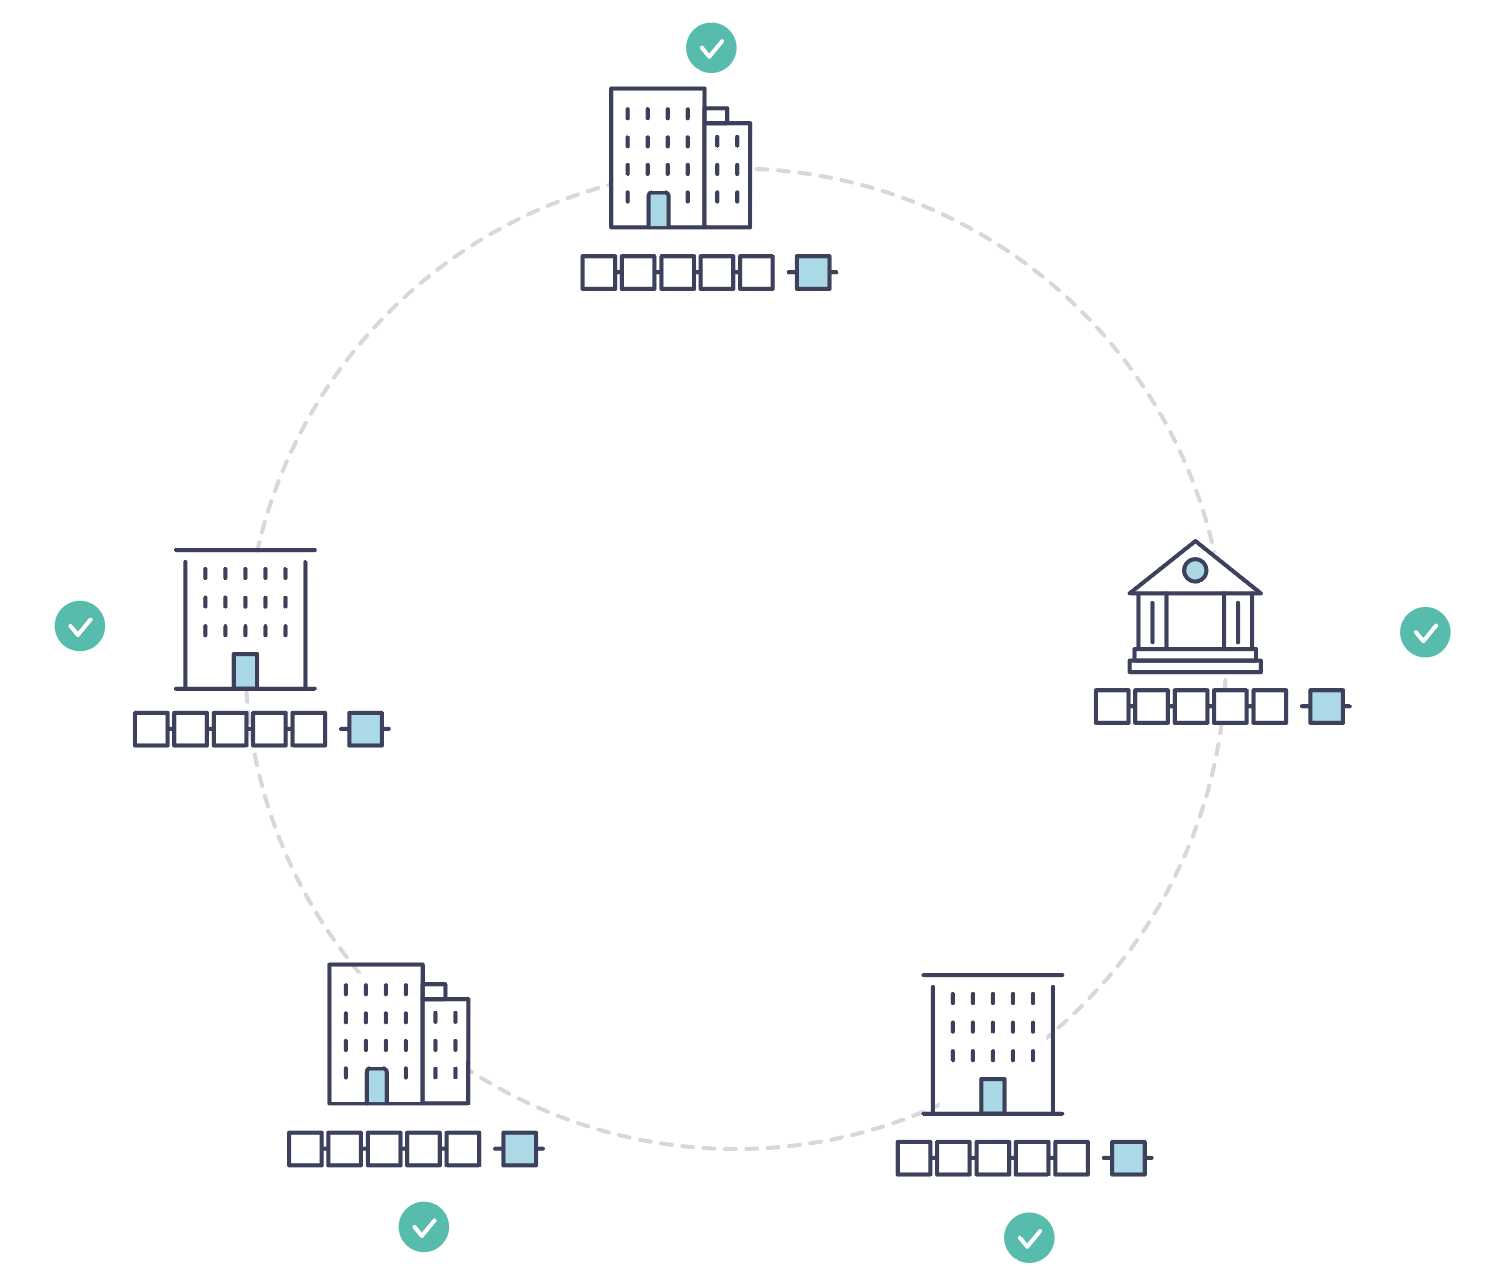
\includegraphics[scale=0.3]{img/future_net.png}
			\caption{Re'tele de afaceri decentralizate\cite{fabricdoc}}
  			\label{fig:decentralised}
  		\end{center}
  		\end{figure}
  		

\chapter{Analiz'a 'si Fundamentare Teoretic'a}
\label{ch:analysis}
Acest capitol prezinta tehnologiile folosite pentru realizarea unei aplicatii decentralizate pentru managementul studiilor clinice.

\section{Cerinte sistem}
Sectiunea prezinta o analiza a sistemului pentru managementul studiilor clinice. Cerintele unui sistem pot fi clasificate in cerinte functionale si non-functionale. Cerintele functionale descriu comportamentul sistemului din punctul de vedere al utilizatorilor. Cerintele non-functionale descriu proprietati si impun constrangeri asupra sistemului.

\subsection{Cerinte functionale}
In continuare sunt prezentate cerintele functionale indeplinite de modulul client al aplicatiei. Aceste functionalitati sunt disponibile pentru utilizatorii sistemului:
\begin{enumerate}
	\item \textbf{Autentificare}: Accesul la funtionalitatile aplicatiei este disponibil doar pentru utilizatorii autentificati. Identitatea utilizatorului are o importanta majora in cadrul retelei blockchain. In acest mod este asigurata posibilitatea urmarii activitatii participantilor si salvarea unui istoric a tuturor operatiilor efectuate de acestia. 
	\item \textbf{Emitere identitate}: Utilizatorii autentificati au nevoie de o identitate emisa de organizatia din care fac parte pentru a putea accesa reteaua. Cu ajutorul acesteia utilizatorii sunt identificati in reteaua blockchain si supusi regulilor de acces la resurse definite in sistem.
	\item \textbf{Creare studiu clinic}: Utilizatorii au posibilitatea de a crea un nou studiu clinic folosind interfata utilizator dupa introducerea informatiilor necesare.
	\item \textbf{Vizualizare studiu clinic}: Ofera posibilitatea utilizatorilor autentificati care au drepturile de acces necesare sa acceseze informatiile despre un studiu clinic si datele legate de activitatea desfasurata in cadrul acestora.
	\item \textbf{Inrolare pacienti}: Posibilitatea de a asocia un pacient la un studiu clinic.
	\item \textbf{Definire formulare}: Cercetatorii pot defini in cadrul unui studiu clinic formulare de colectare a datelor de la pacienti. Aceste formulare ofera cercetatorului flexibilitatea de a defini campuri de text si intrebari cu variante de raspuns relevante pentru studiul clinic.
	\item \textbf{Colectare date}: Folosind formularele definite, cercetatorii au posibilitatea de a colecta date de la un anumit pacient.
	\item \textbf{Management drepturi de acces}: Administratorul unui studiu clinic defineste drepturile de citire sau scriere a utilizatorilor pentru studiul clinic de care este responsabil
	\item \textbf{Management fisier protocol}: Protocolul unui studiu clinic descrie modul de desfasurare al unui studiu clinic. Utilizatorii care detin drepturile de acces necesare pot incarca un fisier de protocol si il pot descarca prin intermediul interfetei utilizator
\end{enumerate}

\subsection{Cerinte non-functionale}
\begin{enumerate}
\item \textbf{}
\end{enumerate}

\chapter{Proiectare de Detaliu 'si Implementare}

'Impreun'a cu capitolul precedent reprezint'a aproximativ 60\% din total.

Scopul acestui capitol este de a documenta aplica'tia dezvoltat'a 'in a'sa fel 'inc\ia t dezvoltarea 'si 'intre'tinerea ulterioar'a s'a fie posibile. 
Cititorul trebuie s'a identifice func'tiile principale ale aplica'tiei din ceea ce este scris aici.
Capitolul ar trebui sa con'tin'a (nu se rezum'a neap'arat la):
\begin{itemize}
 \item schema general'a a aplica'tiei
\item descrierea fiec'arei componente implementate, la nivel de modul
\item diagrame de clase, clase importante 'si metode ale claselor importante.
\end{itemize}


\chapter{Testare 'si Validare}

Aproximativ 5\% din total

\section{Titlu}
\section{Alt titlu}

\chapter{Manual de Instalare 'si Utilizare}

'In sec'tiunea de Instalare trebuie s'a detalia'ti resursele software 'si hardware necesare pentru instalarea 'si rularea aplica'tiei, precum 'si o descriere pas cu pas a procesului de instalare. 
Instalarea aplica'tiei trebuie s'a fie posibil'a pe baza a ceea ce se scrie aici.

'In acest capitol trebuie s'a descrie'ti cum se utilizeaz'a aplica'tia din punct de vedere al utilizatorului, f'ar'a a men'tiona aspecte tehnice interne.
Folosi'ti capturi ale ecranului 'si explica'tii pas cu pas ale interac'tiunii. 
Folosind acest manual, o persoan'a ar trebui s'a poat'a utiliza produsul vostru.

\section{Titlu}
\section{Alt titlu}

\chapter{Concluzii}

Cca. 5\% din total.
Capitolul ar trebui sa con'tin'a (nu se rezum'a neap'arat la):
\begin{itemize}
 \item un rezumat al contribu'tiilor voastre
\item analiz'a critic'a a rezultatelor ob'tinute
\item descriere a posibilelor dezvolt'ari 'si 'imbun'at'a'tiri ulterioare
\end{itemize}


\section{Titlu}
\section{Alt titlu}


%\addcontentsline {toc}{chapter}{Bibliography} 
\bibliographystyle{IEEEtran} 
\bibliography{thesis}%same file name as for .bib

\appendix
\chapter{Profil de conexiune Hyperledger Composer}
\label{app:con}
\begin{verbatim}
{
    "name": "fabric-network",
    "x-type": "hlfv1",
    "version": "1.0.0",
    "peers": {
        "peer0.org1.example.com": {
            "url": "grpc://localhost:7051",
            "eventUrl": "grpc://localhost:7053"
        }
    },
    "certificateAuthorities": {
        "ca.org1.example.com": {
            "url": "http://localhost:7054",
            "caName": "ca.org1.example.com"
        }
    },
    "orderers": {
        "orderer.example.com": {
            "url": "grpc://localhost:7050"
        }
    },
    "organizations": {
        "Org1": {
            "mspid": "Org1MSP",
            "peers": [
                "peer0.org1.example.com"
            ],
            "certificateAuthorities": [
                "ca.org1.example.com"
            ]
        }
    },
    "channels": {
        "composerchannel": {
            "orderers": [
                "orderer.example.com"
            ],
            "peers": {
                "peer0.org1.example.com": {
                    "endorsingPeer": true,
                    "chaincodeQuery": true,
                    "eventSource": true
                }
            }
        }
    },
    "client": {
        "organization": "Org1",
        "connection": {
            "timeout": {
                "peer": {
                    "endorser": "300",
                    "eventHub": "300",
                    "eventReg": "300"
                },
                "orderer": "300"
            }
        }
    }
}
\end{verbatim}

\chapter{Configurare server REST cu utilizatori multiplii}
\label{multiusr}
\begin{verbatim}
export COMPOSER_PROVIDERS='{
  "github": {
    "provider": "github",
    "module": "passport-github",
    "clientID": "[ID]",
    "clientSecret": "[SECRET]",
    "authPath": "/auth/github",
    "callbackURL": "/auth/github/callback",
    "successRedirect": "http://localhost:4200?loggedIn=true",
    "failureRedirect": "/"
  }
}'

export COMPOSER_DATASOURCES='{
    "db": {
        "name": "mydb",
        "connector": "mongodb",
        "database": "mydb",
        "host": "localhost"
    }
}'


composer-rest-server -c admin@clinic-trial-network -n never -m true
\end{verbatim}

\chapter{Modul pentru testarea aplica'tiei client}
\label{app:test}
\begin{verbatim}
describe('OrganisationFormComponent', () => {
  let component: OrganisationFormComponent;
  let fixture: ComponentFixture<OrganisationFormComponent>;

  beforeEach(async(() => {
    TestBed.configureTestingModule({
      imports: [
        FormsModule,
        ReactiveFormsModule,
        AppMaterialModule,
        RouterTestingModule,
        HttpClientModule,
        BrowserAnimationsModule
      ],
      declarations: [OrganisationFormComponent],
      providers:[
        ResearchSiteService,
        SupplyOrganisationService,
        DataService,
        Configuration
      ]
    })
      .compileComponents();
  }));
  beforeEach(() => {
    fixture = TestBed.createComponent(OrganisationFormComponent);
    component = fixture.componentInstance;
    fixture.detectChanges();
  });

  it('should create', () => {
    expect(component).toBeTruthy();
  });
});
\end{verbatim}



\end{document}
